\section{Laboratoire de Pulsipher}

\subsection{Jebble}
\noindent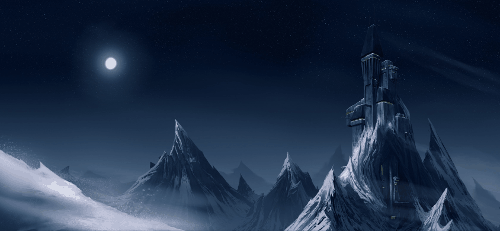
\includegraphics[width=\linewidth]{_img/dos-au-muur/jebble.png}
\'A l'extrémité de la bordure extérieure, complètement gelée à l’image de Hoth, Jebble constituait autrefois le dernier rempart de défence de la République contre les Mandaloriens. Jebble a été le théatre des évènements consernant le Talisman de Muur, Céleste Morne et \nameref{sec:pulsipher}. C’est durant ces évènement que la planète a été bombardé entièrement par la flotte de Cassus Fett afin d’éviter la contagion des Rakghouls. Ce bombardement a fait fondre les glaces de Jebble et les installation de Pulsipher ont coulé dans les eaux bouillonnates qui ont regelé par dessus.

Il y a plus de 1~000~ans des mineurs qui cherchaient a exploiter les ressources de la planète, sont tombé sur les installation de Pulsipher, y ont trouvé l'oubliette de Dreya qu'ils ont vendu en tant que « Boite de Jebble ».

Depuis la planète Jebble a sombré dans le déintéret le plus complet pour le reste de la galaxie.

\subsection{Astroport de Kriloo City}



%   L'épisode suivant se passe sur Jebble dans le labo du professeur Pulcipher. Où l'on apprend ce qu'il s'est passé pendant le voyage de retour. On trouve aussi des information sur l'oubliette de Dreypa et l'on a des piste sur l'endroit où elle se trouve. On entend notement parler de Céleste Morne.
%   Ici une idée est qu'au moment de quitté la planète pour l'étape suivante, les héros se retrouvent pris au piège par des troupes de l'empire qui on pris leur vaisseau en otage. Histoire de varier l'aventure. On peut même se mettre une petite baston spaciale.
%   Il faudra ensuite forcer les héros à retourner à leur QG (alliance rebelle ou empire) pour réparation et pour compte rendu.

%   Dans l'épisode suivant, le rebelles apprennent qu'on aurait vu le talisman sur une certaine lune de Jesaispasou et les soldats de l'empire apprenne qu'ils vont tendre un piège à l'alliance sur un lune de Jesaispasou.
%   Grossomerdo, Celeste se pointe et calme tout le monde, obligé de battre en retraite et de trouver un plan pour enfermer Celeste dans l'oubliette de Dreypa ou pour lui virer le Talisman avant d'enfermer ce dernier dans l'oubliette. Ou se trouve l'oubliette ? Quel est le plan ?